\documentclass{beamer}

\usefonttheme{serif}
\usepackage{charter}

\usepackage[utf8]{inputenc}
\usepackage[english]{babel}
\usepackage{listings}
\usepackage{graphicx}
 \usepackage{epstopdf}

\setbeamertemplate{navigation symbols}{}
\setbeamertemplate{footline}[frame number]{}
%\setbeamertemplate{footline}{\hfill\insertframenumber~\vrule~\inserttotalframenumber}
\lstset{
  stepnumber=1,
  breaklines=true,
  basicstyle=\ttfamily\scriptsize,
  numberstyle=\tiny,
  commentstyle=\color{gray},
  showstringspaces=false,
  keepspaces=true,
  escapeinside=\#\#
}

\renewcommand\big[1]{
  \begin{center}
    \Large{#1}
  \end{center}
}

\begin{document}

\begin{frame}
  \centering\Huge{awk}
\end{frame}

\begin{frame}
  \big{demo.txt}
  \lstinputlisting{demo.txt}
\end{frame}

\begin{frame}
  \centering\Huge{Principle \#1}
  \big{Patterns and actions}
\end{frame}

\begin{frame}[fragile]
  \big{Patterns and actions}

  \begin{itemize}
    \item A awk program is a list of patterns and actions to execute;
    \item Patterns are tried in order for every line of input;
    \item More than one pattern can match.
  \end{itemize}

  \begin{lstlisting}
    pattern_1 { actions_1 }
    pattern_2 { actions_2 }
    ...
    pattern_k { actions_k }
  \end{lstlisting}
\end{frame}

\begin{frame}[fragile]
  \big{Execution model}

  \begin{lstlisting}
    for each $line {
      for each $pattern, $action {
        if $line matches $pattern {
          execute $action
        }
      }
    }
  \end{lstlisting}
\end{frame}

\begin{frame}[fragile]
  \big{Examples}
  \begin{lstlisting}
    /erlang/                     { erl_projects++ }
    length($3) < 5               { print $1, $3 }
    $2 == "backend" && $3 == "c" { print $0 }
  \end{lstlisting}
\end{frame}

\begin{frame}[fragile]
  \big{Demo}
  \begin{lstlisting}
    > awk '/erlang/ { erl_projects++ }' demo.txt
    [no output]
    #\pause#

    > awk 'length($3) < 5 { print $1, $3 }' demo.txt
    rtb-trader ruby
    iplist-service c
    #\pause#

    > awk '$2=="backend" && $3=="c" { print $0 }' demo.txt
    iplist-service  backend     c
  \end{lstlisting}
\end{frame}

\begin{frame}[fragile]
  \big{Two special patterns}

  \begin{lstlisting}
    BEGIN { /* run before any line is processed */ }
    END   { /* run after all lines are processed */ }
  \end{lstlisting}

  \begin{center}Useful for initialization and reporting.\end{center}
\end{frame}

\begin{frame}[fragile]
  \big{Example}
  \begin{lstlisting}
    > awk '/erlang/ { p++ } END { print p }' demo.txt
    2
  \end{lstlisting}
\end{frame}

\begin{frame}
  \centering\Huge{Principle \#2}
  \big{Abbreviate common use cases}
\end{frame}

\begin{frame}[fragile]
  \big{No pattern}

  If no pattern is specified, all lines match.

  \begin{lstlisting}
    > awk '{print $1}' demo.txt
    rtb-gateway
    rtb-trader
    iplist-service
    identifyd
    rtb-delivery
  \end{lstlisting}
\end{frame}

\begin{frame}[fragile]
  \big{No action}

  If no action is specified, the whole line is printed.

  \begin{lstlisting}
    > awk '/data|backend/' demo.txt
    rtb-gateway     backend     erlang
    iplist-service  backend     c
    identifyd       data        scala
    rtb-delivery    backend     erlang
  \end{lstlisting}
\end{frame}

\begin{frame}[fragile]
  \big{Print without arguments}

  \texttt{print} without arguments prints the whole line.

  \begin{lstlisting}
    > awk '$2 == "data" || $3 == "c" { print }' demo.txt
    iplist-service  backend     c
    identifyd       data        scala
  \end{lstlisting}
\end{frame}

\begin{frame}[fragile]
  \big{Variables initialization}

  Variables are automatically initialized when first used.

  \begin{lstlisting}
    > cat demo.txt \
    | awk '{c[$3]++} END { for (l in c) print l, c[l] }'
    scala 1
    erlang 2
    ruby 1
    c 1
  \end{lstlisting}
\end{frame}

\begin{frame}
  \centering\Huge{Principle \#3}
  \big{Allow custom formatting}
\end{frame}

\begin{frame}[fragile]
  \big{Record separator}

  \begin{itemize}
    \item By default, records are separated by newlines.
    \item Can be modified through \texttt{RS} variable.
  \end{itemize}\pause

  \begin{lstlisting}
    > echo "a b::c d" | awk -v RS=:: '{print $1}'
    a
    c
    #\pause#
    > echo "a b::c d" | awk 'BEGIN { RS="::" } {print $2}'
    b
    d
  \end{lstlisting}
\end{frame}


\begin{frame}[fragile]
  \big{Field separator}

  \begin{itemize}
    \item By default, fields are separated by whitespace.
    \item Can be modified through \texttt{FS} variable.
  \end{itemize}\pause

  \begin{lstlisting}
    > echo -e "a,b\nc,d" | awk -F, '{print $1}'
    a
    c
    #\pause#
    > echo -e "a,b\nc,d" | awk -v FS=, '{print $1}'
    a
    c
    #\pause#
    > echo -e "a--b\nc-d" | awk 'BEGIN {FS="-+"} {print $2}'
    b
    d
  \end{lstlisting}
\end{frame}

\begin{frame}[fragile]
  \big{Output separators}

  \begin{lstlisting}
    > echo -e "a b\nc d" | \
      awk -v OFS='|' -v ORS=']' '{print $1, $2}'
    a|b]c|d]
    #\pause#
    > echo -e "a b\nc d" | \
      awk -v OFS='|' -v ORS=']' '{print $0}'
    a b]c d]
  \end{lstlisting}
\end{frame}

\begin{frame}
  \centering\Huge{Principle \#4}
  \big{Don't be too different}
\end{frame}

\begin{frame}[fragile]
  \big{Awk statements have a C-like syntax}

  \begin{lstlisting}
    if (expr) stmt [else stmt]
    while (expr) stmt
    for (expr; expr; expr) stmt
  * for (var in array) stmt
    do stmt while (expr)
    break
    continue
    { [stmt ...] }
    expr
  * print [expr-list] [>expr]
    printf format [..., expr-list] [>expr]
    return [expr]
  * next (skip all remaining patterns, goto next line)
  * nextfile (skip to next file)
  * delete array[expr]
  * delete array
    exit [expr]
  \end{lstlisting}
  \scriptsize{Source: OpenBSD awk(1) man page}
\end{frame}

\begin{frame}[fragile]
  \big{JavaScript has Awk-like function syntax}

  \begin{lstlisting}
    function foo(a, b, c) {
      ...;
      return a;
    }
  \end{lstlisting}

  \scriptsize{(You declare functions at the top-level, i.e., with patterns.)}
\end{frame}

\begin{frame}[fragile]
  \big{Awk has common functions}
  \begin{lstlisting}
     atan2(y, x)         gsub(r, t, s)
     cos(x)              index(s, t)
     exp(x)              length(s)
     int(x)              match(s, r)
     log(x)              split(s, a, fs)
     rand()              sprintf(fmt, expr, ...)
     sin(x)              sub(r, t, s)
     sqrt(x)             substr(s, m, n)
     srand(expr)         tolower(str)
                         toupper(str)
  \end{lstlisting}

  \scriptsize{Source: OpenBSD awk(1) man page}
\end{frame}

\begin{frame}
  \centering\Huge{Principle \#5}
  \big{A language that grows on you}
\end{frame}

\begin{frame}
  \big{A tool that grows with you}

  \begin{itemize}
    \item awk can slowly be incorporated in your day-to-day;
    \item as you use it, you'll discover more places where it's useful;
    \item over time, it reduces the number of times you have to use Python to do a one-off task.
  \end{itemize}
\end{frame}

\begin{frame}
  \centering\Huge{/awk}
\end{frame}

\begin{frame}
  \centering\Huge{Bonus content!}
  \big{Simple re-implementations of Unix tools in awk}
\end{frame}

\begin{frame}[fragile]
  \big{\texttt{cat(1)}}
  \pause
  \begin{lstlisting}
    > awk '{print}' demo.txt
    #\pause#
    > awk 1 demo.txt
  \end{lstlisting}
\end{frame}

\begin{frame}[fragile]
  \big{\texttt{grep(1)}}
  \pause
  \begin{lstlisting}
    > awk '/PATTERN/' demo.txt
  \end{lstlisting}
\end{frame}

\begin{frame}[fragile]
  \big{\texttt{wc(1)}}
  \pause
  \begin{lstlisting}
    > awk '{nl++; nc += length($0)+1; nw += NF}
           END { print nl, nw, nc, FILENAME; }' demo.txt
    #\pause#
    > awk '{nc += length($0)+1; nw += NF}
           END { print NR, nw, nc, FILENAME; }' demo.txt
  \end{lstlisting}
\end{frame}

\begin{frame}[fragile]
  \begin{center}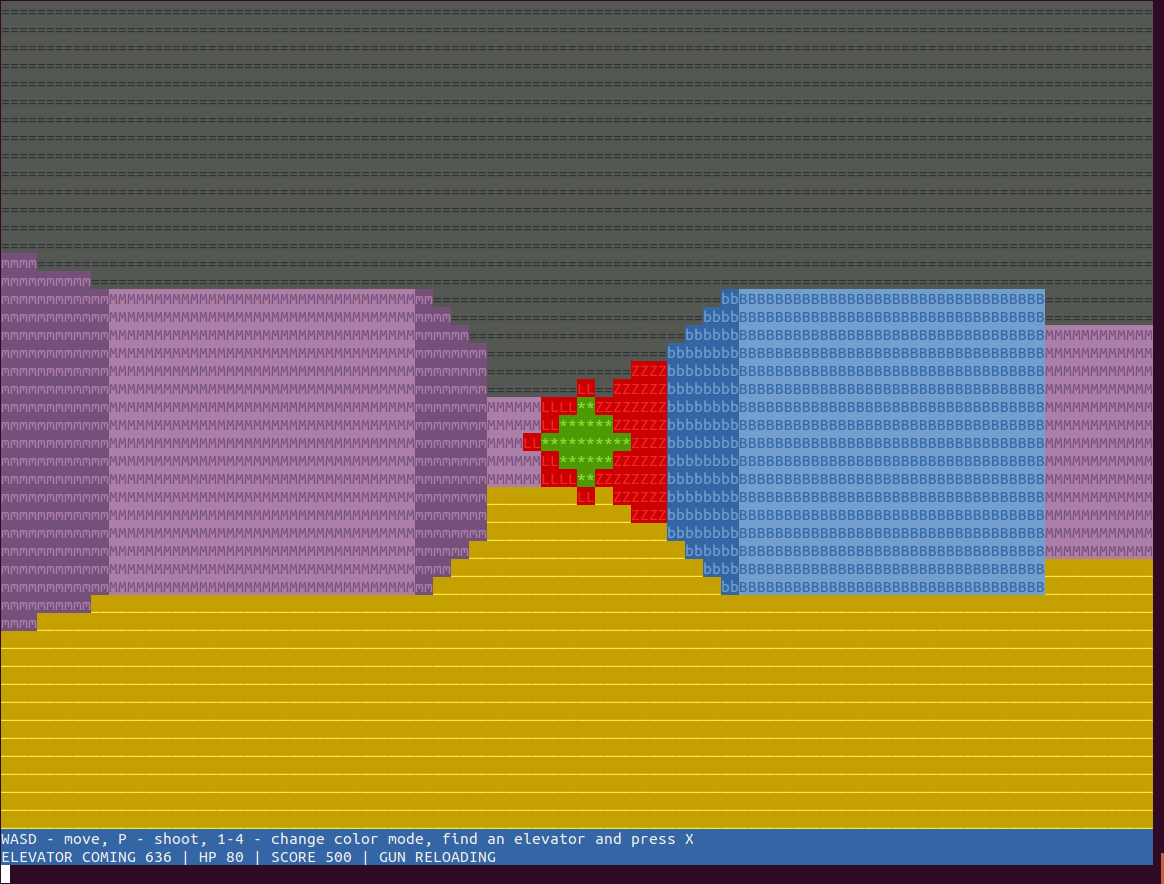
\includegraphics[scale=.22]{awkaster.png}\end{center}
  \scriptsize{Source: \url{https://github.com/TheMozg/awk-raycaster}}
\end{frame}

\end{document}
